\section{Web statico e Web dinamico}

    Il modello che abbiamo analizzato finora, basato sul concetto di ipertesto distribuito, ha una natura essenzialmente statica. Anche se l’utente può percorrere dinamicamente l’ipertesto in modi molto diversi, l’insieme dei contenuti è prefissato staticamente.
    
    \vspace{3mm}
    
    Una generica \textbf{architettura dinamica} presenta numerosi vantaggi ma soffre anche di diversi problemi. Ci sono problemi di prestazioni: ogni volta che viene invocata un programma si crea un processo che viene distrutto alla fine dell’elaborazione; in alternativa, ogni programma deve reimplementare tutta una serie di parti comuni (mancanza di moduli di base accessibili a tutti i programmi lato server: accesso al DB, logica di interpretazione delle richieste HTTP e di costruzione delle risposte, gestione dello stato, etc). Inoltre, abbiamo scarse garanzie sulla sicurezza.
    
    \vspace{3mm}
    
    Per ovviare al penultimo punto si potrebbe realizzare un solo programma che implementa le funzionalità. In questo modo però si ha un’applicazione monolitica e si perdono i vantaggi della modularità. Gli altri problemi rimangono invariati.
        
    \subsection{Containers e Application Servers}
        
    Il \textbf{contenitore} si preoccupa di fornire i servizi di cui le applicazioni hanno bisogno. Un esempio di container è Tomcat. Il container è composto da servlets.
    
    L'\textbf{Application Server} si interfaccia al Web Server (browser), spesso connettendosi anche ad un database.
    
    \begin{itemize}
        
        \item Interfacciamento con il Web Server
        
        \item Gestione del tempo di vita (attivazione on-demand delle funzioni)
        
        \item Interfacciamento con il database
        
        \item Gestione della sicurezza
        
        \item Si ha così una soluzione modulare in cui le funzionalità ripetitive vengono
        portate a fattor comune
        
        \item Un ambiente di questo tipo prende il nome di application server
    \end{itemize}    

    L’interazione tra un Client e un Server può essere infatti di due tipi:
    
    \begin{itemize}
        \item \textbf{Stateful}: esiste stato dell’interazione e quindi l’n-esimo
        messaggio può essere messo in relazione con gli n-1
        precedenti
        
        \item \textbf{Stateless}: non si tiene traccia dello stato, ogni messaggio è
        indipendente dagli altri
    \end{itemize}
    
    In termini generali, un’interazione stateless è “\textit{feasible}” senza generare grossi problemi solo se il protocollo applicativo è progettato con operazioni idempotenti. Operazioni idempotenti producono sempre lo stesso risultato, indipendentemente dal numero di messaggi M ricevuti dal server stesso. Ad esempio, un server fornisce sempre la stessa risposta \(R\) a un messaggio \(M\).
    
    \vspace{3mm}
    
    Non tutte le applicazioni possono fare a meno dello stato. Esempio banale: se è prevista un’autenticazione.
    
    \vspace{3mm}
    
    Parlando di applicazioni Web è possibile classificare lo stato in modo più preciso:
    
    \begin{itemize}
        \item \textbf{Stato di esecuzione} (insieme dei dati parziali per una
        elaborazione): rappresenta un avanzamento in una
        esecuzione; per sua natura è uno stato volatile; può essere
        mantenuto in memoria lato server come stato di uno o più
        oggetti
        
        \item \textbf{Stato di sessione} (insieme dei dati che caratterizzano una
        interazione con uno specifico utente): la sessione viene
        gestita di solito in modo unificato attraverso l’uso di istanze. La conversazione rappresenta una sequenza di pagine di senso
        compiuto (ad esempio, l’insieme delle pagine necessarie per comperare
        un prodotto). E' univocamente definita dall'insieme delle pagine che la compongono e
        dall’insieme delle interfacce di input/output per la comunicazione tra le
        pagine (flusso della conversazione) di oggetti specifici (supporto a oggetti sessione)
        
        \item \textbf{Stato informativo persistente} (ad esempio gli ordini
        inseriti da un sistema di e-commerce): viene normalmente
        mantenuto in una struttura persistente come un database 
    \end{itemize}
    
    La \textbf{sessione} rappresenta lo stato associato ad una sequenza di pagine visualizzate da un utente: contiene tutte le informazioni necessarie durante l’esecuzione (informazioni di sistema: IP di provenienza, lista delle pagine visualizzate, etc); informazioni di natura applicativa: nome e cognome, username, quanti e quali prodotti ha inserito nel carrello per un acquisto).
    
    \vspace{3mm}
    
    Lo \textbf{scope di sessione} è dato da: tempo di vita della interazione utente (lifespan) eccessibilità: usualmente concesso alla richiesta corrente e a tutte le richieste successive provenienti dallo stesso browser.
    
    \vspace{3mm}
    
    La \textbf{conversazione} rappresenta una sequenza di pagine di senso compiuto (ad esempio, l’insieme delle pagine necessarie per comperare
    un prodotto). E' univocamente definita dall’insieme delle pagine che la compongono e dall’insieme delle interfacce di input/output per la comunicazione tra le pagine (flusso della conversazione) 
    
    \vspace{3mm}
    
    Ci sono due tecniche di base per gestire lo stato, non necessariamente alternative ma integrabili: utilizzo del meccanismo dei \textbf{cookie} (storage lato client), gestione di uno stato sul server per ogni utente collegato (sessione server-side).
    
    \subsection{Architettura Multilivello}
    
    Sviluppare applicazioni secondo una logica ad oggetti e/o a componenti significa scomporre l’applicazione in blocchi, servizi e
    funzioni. E' molto utile separare logicamente le funzioni necessarie in una struttura multilivello (multi-tier) al fine di fornire astrazioni via via più complesse e potenti a partire da funzionalità più elementari. 
    
    \begin{center}
        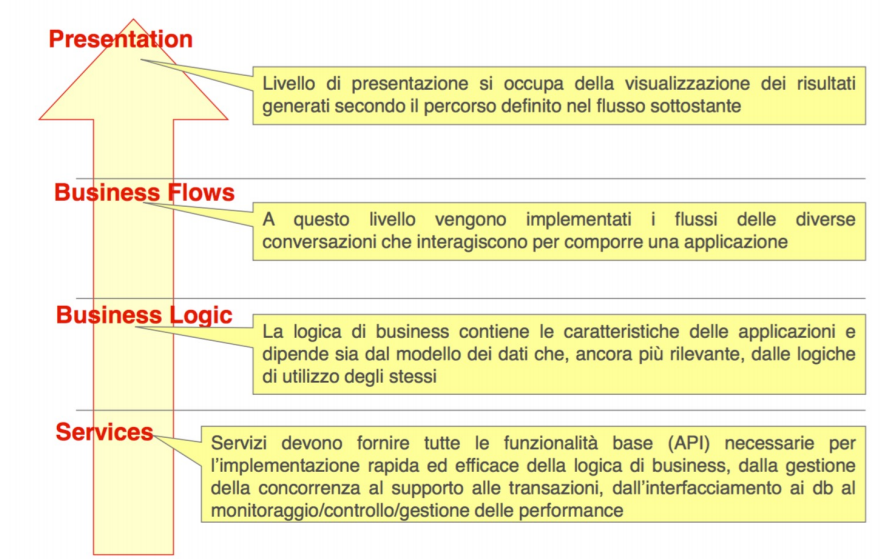
\includegraphics[scale=0.5]{images/ApplicationServer.png}
    \end{center}
    
    Nel tempo si è affermata una classificazione indipendente dalla implementazione tecnologica, basata su una struttura a 4 livelli principali. Questa struttura non fornisce dettagli implementativi, non specifica quali moduli debbano essere implementati client-side o server-side, ne nessuna altra specifica tecnica: è una architettura essenzialmente logico-funzionale.
    
    • Communications Support
    
    • Lifecycle Management
    
    • Multithreading Support
    
    • Declarative Security
    
    • JSP Support
    
    \subsubsection{Java Models}
    
    Nel progetto di applicazioni Web in Java, due sono i modelli di ampio uso e di riferimento: \textbf{Model 1} e \textbf{Model 2}. Il primo modello sposta la maggior parte della logica applicativa da JSP e le Servlets alle classe Java, come i JavaBeans. Il secondo modello separa ancora di più i modelli e le servlets dalle view.
    
    \subsubsection{MVC}
    
    Architettura adatta per applicazioni Web interattive.
    
    \vspace{3mm}
    
    \textbf{Model} – rappresenta livello dei dati, incluse operazioni per accesso e
    modifica. Model deve notificare le view associate quando viene modificato
    e deve supportare:
    
    \begin{itemize}
        \item La possibilità per la view di interrogare stato di model
        \item La possibilità per il controller di accedere alle funzionalità incapsulate dal model
    \end{itemize}

    \textbf{View} – si occupa del rendering dei contenuti del model. Accede ai dati
    tramite il model e specifica come dati debbano essere presentati.
    
    \begin{itemize}
        \item Aggiorna la presentazione dei dati quando il model cambia
        \item Gira l’input dell’utente verso il controller
    \end{itemize}
    
    \textbf{Controller} – definisce il comportamento dell’applicazione.
    
    \begin{itemize}
        \item Fa dispatching di richieste utente e seleziona la view per la presentazione.
        
        \item Interpreta l’input dell’utente e lo mappa su azioni che devono essere eseguite
        dal model (in una GUI stand-alone, input come click e selezione menu; in una
        applicazione Web, richieste HTTP GET/POST).
    \end{itemize}